\graphicspath{ {02-CoordinateSystems/Figures/} }

\section{Coordinate systems}

\subsection{Laboratory coordinate system}

The origin of the LhARA coordinate system, the ``laboratory coordinate
system'' or ``laboratory reference frame'', is at the position of the
laser focus at the position of the laser-target interaction.
The $z$ axis is horizontal and parallel to the nominal capture axis,
pointing in the downstream direction.
The $y$ axis points vertically upwards, and the $x$ axis completes a
right-handed orthogonal coordinate system. 

Unit vectors along the $x$, $y$ and $z$ axes are $\bm{i}$, $\bm{j}$
and $\bm{k}$ respectively.
The position of the reference particle, its momentum and energy are
described as functions of the distance it has travelled from the origin
of coordinates to its current position.
The distance travelled is defined to be $s$, making the position,
$\bm{r}_0$, momentum, $\bm{p}_0$, and energy, $E_0$, of the
reference particle at position $s$:
\begin{eqnarray}
  \bm{r}_0 & = & \bm{r}_0(s)\, ;           \nonumber \\
  \bm{p}_0 & = & \bm{p}_0(s)\, {\rm ; and}           \\
       E_0 & = &      E_0(s)\, .           \nonumber
\end{eqnarray}
The time, $t$, at which the reference particle is at $s$ is also a
function of $s$:
\begin{eqnarray}
        t  & = & t(s) = \frac{c}{s} \frac{c p_0}{E_0}\, ; 
\end{eqnarray}
where $p_0=\left|\bm{p}_0\right|$ and $c$ is the speed of light.

\subsection{Reference particle local coordinate system}

A coordinate system defined relative to the position of the reference
particle, the ``reference particle local coordinate'' (RPLC) system,
may be defined using the direction in which the particle is
travelling. 
The position of the particle defines the origin of the RPLC system,
see figure~\ref{fig:RPLC}.
\begin{figure}
  \begin{center}
    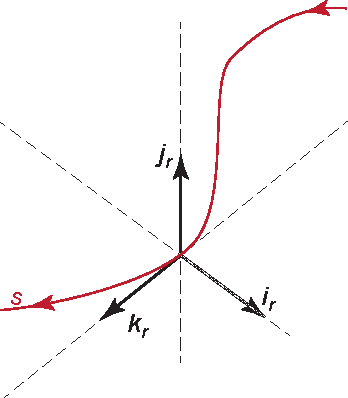
\includegraphics[width=0.55\linewidth]{RPLC.pdf}
  \end{center}
  \caption{
    Reference particle local coordinate system.
    The trajectory of the reference particle is shown as the red line.
    The distance the reference particle has travelled, measured from
    the origin of coordinates in the laboratory frame, is labelled
    $s$.
    The origin of the RPLCs is coincident with the position of the
    reference particle.
    The directions of unit vectors along each of three righthanded,
    orthogonal coordinate axes are shown as black arrows labelled
    $\bm{i}_0$, $\bm{j}_0$, and $\bm{j}_0$. 
  }
  \label{fig:RPLC}
\end{figure}

The tangent to the reference particle trajectory at $s$ defines the
$z_{\rm RPLC}$ axis with unit vector $\bm{k}_{\rm RPLC}$.
In the laboratory frame, the presence of local electric or magnetic
fields may cause the reference particle's trajectory to change.
In the neighbourhood of the particle, the curved trajectory may be
described in terms of an arc of a circle.
The $x_{\rm RPLC}$ axis (with unit vector $\bm{i}_{\rm RPLC}$) is then
taken to be in the direction pointing towards the centre of the
circle. 
The third coordinate axis, $y_{\rm RPLC}$, is defined to complete the
right-handed orthogonal coordinate system; the unit vector along the
$y_{\rm RPLC}$ axis being given by
$\bm{j}_{\rm RPLC} = \bm{k}_{\rm RPLC} \times \bm{i}_{\rm RPLC}$.

The trajectory of the reference particle will be a straight line as it
traverses a drift space or when the particle's energy is increased (or
decreased) through an electric field applied parallel to its direction
of motion.
In such cases the RPLC axes are taken to coincide with either the
laboratory coordinate system or the RPLC system defined at the exit of
the beam-line element that preceded the drift space or accelerating
element.

\subsection{Transforming to and from reference particle local
            coordinates to laboratory coordinates}
            
In the RPLC system, the trajectory of the reference particle,
$\bm{R}_0$, is:
\begin{equation}
  \bm{R}_0(s) = \bm{0}\,.
\end{equation}
The position of a test particle in the RPLC frame, $\bm{R}$, is
described with reference to the position of the reference particle.
In the laboratory frame, the position of the test particle is:
\begin{equation}
  \bm{r}(s) = \bm{r}_0(s) + \bm{\delta r}(s) \,;
\end{equation}
where:
\begin{equation}
  \bm{\delta r}(s) = \underline{\underline{R}}(s) \bm{R}(s) \,{\rm ; and}
\end{equation}
$\underline{\underline{R}}(s)$ is a rotation matrix that takes
the RPLCs at $s$ to the laboratory frame coordinates.

In the laboratory frame, the unit vectors $\bm{i}_{\rm RPLC}$,
$\bm{j}_{\rm RPLC}$ and $\bm{k}_{\rm RPLC}$ are given by:
\begin{eqnarray}
  \bm{i}_{\rm RPLC} & = & \begin{pmatrix} i_{rx} \\ i_{ry} \\  i_{rz} \\ \end{pmatrix} \,;           \nonumber \\
  \bm{j}_{\rm RPLC} & = & \begin{pmatrix} j_{rx} \\ j_{ry} \\  j_{rz} \\ \end{pmatrix} \,{\rm ; and}           \\
  \bm{k}_{\rm RPLC} & = & \begin{pmatrix} k_{rx} \\ k_{ry} \\  k_{rz} \\ \end{pmatrix} \,.           \nonumber
\end{eqnarray}
The rotation matrix, $\underline{\underline{R}}$, may now be written:
\begin{equation}
  \underline{\underline{R}}(s) =
    \begin{bmatrix}
      i_{{\rm RPLC}x} & j_{{\rm RPLC}x} & k_{{\rm RPLC}x} \\
      i_{{\rm RPLC}y} & j_{{\rm RPLC}y} & k_{{\rm RPLC}y} \\
      i_{{\rm RPLC}z} & j_{{\rm RPLC}z} & k_{{\rm RPLC}z}
    \end{bmatrix} \,.
\end{equation}
